\documentclass[a4paper,12pt,twocolumn,landscape]{article}

\usepackage{FabZ}
\usepackage{vecteurs}

\usepackage{geometry}
\geometry{hmargin=0.5cm,vmargin=1.5cm}

%\setlength{\headheight}{0pt}
%\pagestyle{fancyplain}
%\fancyhf{}
%\lhead[]{\textbf{TD Vecteurs}}
%\chead[]{}
%\rhead[]{}
%
%\lfoot[]{}
%\cfoot[]{}
%\rfoot[]{}
%%\rfoot[]{Page \thepage~ sur \pageref{LastPage}}

\fancypagestyle{firststyle}
{
	\setlength{\headheight}{0em}
	\fancyhf{}
	\lhead[]{\textbf{Repérage dans le plan}}
	\chead[]{}
	\rhead[]{\textbf{Repérage dans le plan}}
%	\lhead[]{\textbf{Devoir sur table n°1}}
%	\chead[]{Jeudi 26 septembre 2013}
%	\rhead[]{Géométrie plane, calculs sur les fractions}

	\lfoot[]{}
	\cfoot[]{}
	\rfoot[]{}
%	\rfoot[]{Page \thepage~ sur \pageref{LastPage}}
}

\fancypagestyle{vide}
{
	\setlength{\headheight}{0em}
	\pagestyle{fancyplain}
	\def\headrulewidth{0em}
	\fancyhf{}
	\lhead[]{}
	\chead[]{}
	\rhead[]{}
	
	\lfoot[]{}
	\cfoot[]{}
	\rfoot[]{}
%	\rfoot[]{Page \thepage~ sur \pageref{LastPage}}
}

\usetikzlibrary{fadings}
\newcommand{\Fin}{node[xshift=-1.5ex,rotate=10]{F}
node[rotate=170]{i}
node[xshift=1.5ex,rotate=45]{n}}

\newcommand{\bonnesvacances}{node[xshift=0ex,rotate=10]{B}
node[xshift=1*1.5ex,rotate=170]{o}
node[xshift=2*1.5ex,rotate=45]{n}
node[xshift=3*1.5ex,rotate=128]{n}
node[xshift=4*1.5ex,rotate=75]{e}
node[xshift=5*1.5ex,rotate=130]{s}
node[xshift=6*1.5ex,rotate=85]{~}
node[xshift=7*1.5ex,rotate=128]{v}
node[xshift=8*1.5ex,rotate=43]{a}
node[xshift=9*1.5ex,rotate=4]{c}
node[xshift=10*1.5ex,rotate=145]{a}
node[xshift=11*1.5ex,rotate=5]{n}
node[xshift=12*1.5ex,rotate=25]{c}
node[xshift=13*1.5ex,rotate=105]{e}
node[xshift=14*1.5ex,rotate=45]{s}
}

\begin{document}
\begin{minipage}{0.45\textwidth}
\thispagestyle{firststyle}
%\paragraph*{Exercice}~\\% \hfill \emph{4~points}~\\

\vspace*{2em}

%\input{triangle-milieu-milieu-1}\\

\paragraph{Exercice~1} Lire les coordonnées des points suivants~: 

\begin{minipage}{0.75\textwidth}
\begin{center}
%\fbox{
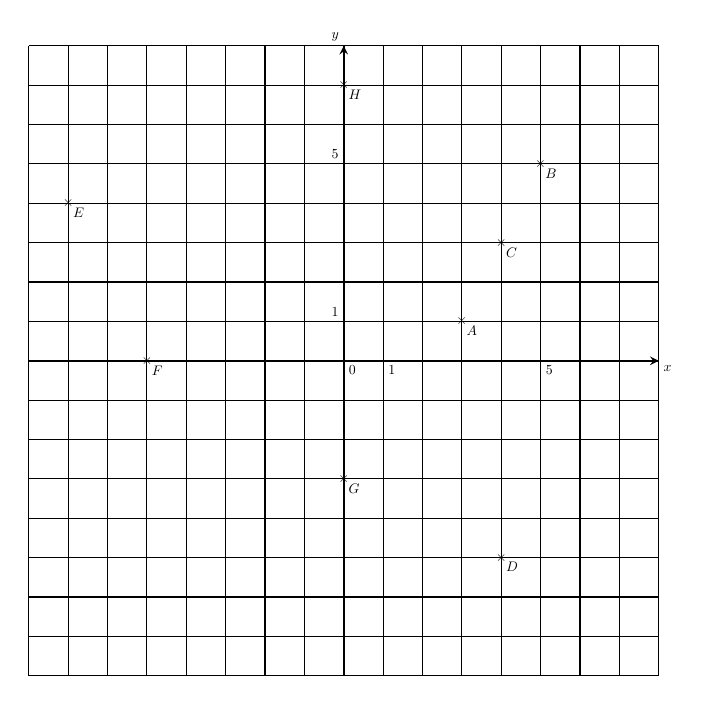
\begin{tikzpicture}[scale=0.5,every node/.style={scale=0.5}]
	%Points
	\coordinate(O)at(0,0);
	\coordinate(I)at(1,0);
	\coordinate(J)at(0,1);
	\coordinate(xstart)at(-8,0);
	\coordinate(xend)at(8,0);
	\coordinate(ystart)at(0,-8);
	\coordinate(yend)at(0,8);
	\coordinate(A)at(3,1);
	\coordinate(B)at(5,5);
	\coordinate(C)at(4,3);
	\coordinate(D)at(4,-5);
	\coordinate(E)at(-7,4);
	\coordinate(F)at(-5,0);
	\coordinate(G)at(0,-3);
	\coordinate(H)at(0,7);
	%Étiquettes
%	\draw (I) node[below right] {$1$};
%	\draw (J) node[above left] {$1$};
	\draw (xend) node[below right] {$x$};
	\draw (yend) node[above left] {$y$};	
	%%%%%%%%%%%%%%%%%%%%%%%%%%%%%%%%%%%%
	%Axes
	\draw [thick] (xstart) -- (xend);
	\draw [thick] (ystart) -- (yend);
	%Flèches
%	\draw [>=stealth,->] (O) -- (I);
%	\draw [>=stealth,->] (O) -- (J);
	\draw [>=stealth,->] (O) -- (xend);
	\draw [>=stealth,->] (O) -- (yend);
	%Grille
	\draw [thin] (-8,-8)grid(8,8);
	%%%%%%%%%%%%%%%%%%%%%%%%%%%%%%%%%%%%
	%étiquettes
	\foreach \point in {A, ..., H}
		\draw(\point)node{$\times$};
	\foreach \point in {A, ..., H}
		\draw(\point)node[below right]{$\point$};	
	\foreach \r in {0, 1, 5}
    	\draw[thick, below right] (\r,0) node{\r};
	\foreach \r in {1, 5}
    	\draw[thick, above left] (0,\r) node{\r};
\end{tikzpicture}
%}
\end{center}
\end{minipage}
\begin{minipage}{0.2\textwidth}
	\begin{enumerate}[]
		\item $A(~~~~~,~~~~~)$
		\item $B(~~~~~,~~~~~)$
		\item $C(~~~~~,~~~~~)$
		\item $D(~~~~~,~~~~~)$
		\item $E(~~~~~,~~~~~)$
		\item $F(~~~~~,~~~~~)$
		\item $G(~~~~~,~~~~~)$
		\item $H(~~~~~,~~~~~)$
	\end{enumerate}
\end{minipage}

\paragraph{Exercice~2} Placer un point connaissant ses coordonnées~:

\begin{minipage}{0.75\textwidth}
\begin{center}
%\fbox{
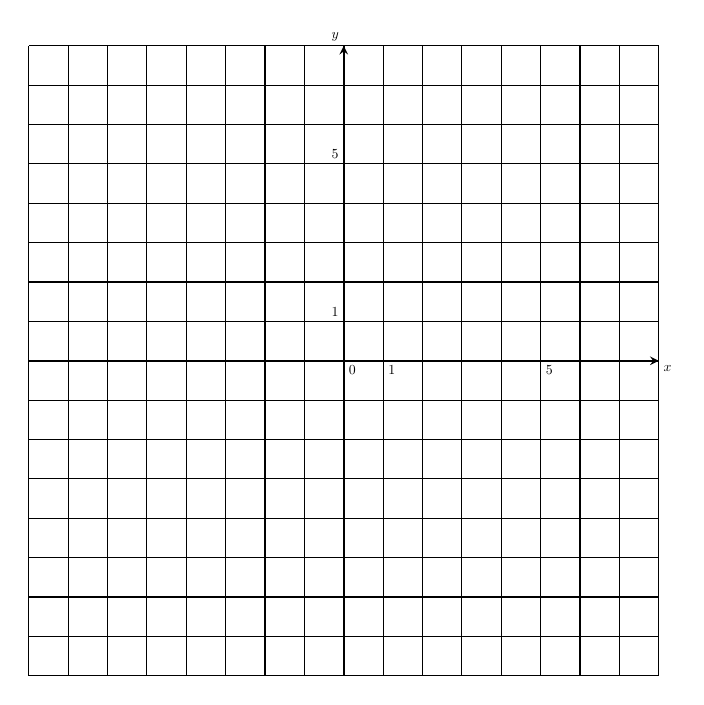
\begin{tikzpicture}[scale=0.5,every node/.style={scale=0.5}]
	%Points
	\coordinate(O)at(0,0);
	\coordinate(I)at(1,0);
	\coordinate(J)at(0,1);
	\coordinate(xstart)at(-8,0);
	\coordinate(xend)at(8,0);
	\coordinate(ystart)at(0,-8);
	\coordinate(yend)at(0,8);
	\coordinate(A)at(5,3);
	\coordinate(B)at(-2,3);
	\coordinate(C)at(-2,-4);
	\coordinate(D)at(6,2);
	\coordinate(E)at(7,-4);
	\coordinate(F)at(6,0);
	\coordinate(G)at(0,3);
	\coordinate(H)at(0,-7);
	%Étiquettes
%		\draw (I) node[below right] {$1$};
%		\draw (J) node[above left] {$1$};
	\draw (xend) node[below right] {$x$};
	\draw (yend) node[above left] {$y$};	
	%%%%%%%%%%%%%%%%%%%%%%%%%%%%%%%%%%%%
	%Axes
	\draw [thick] (xstart) -- (xend);
	\draw [thick] (ystart) -- (yend);
	%Flèches
%		\draw [>=stealth,->] (O) -- (I);
%		\draw [>=stealth,->] (O) -- (J);
	\draw [>=stealth,->] (O) -- (xend);
	\draw [>=stealth,->] (O) -- (yend);
	%Grille
	\draw [thin] (-8,-8)grid(8,8);
	%%%%%%%%%%%%%%%%%%%%%%%%%%%%%%%%%%%%
	%étiquettes
	
% Réponses
%	\foreach \point in {A, ..., H}
%		\draw(\point)node{$\times$};
%	\foreach \point in {A, ..., H}
%		\draw(\point)node[below right]{$\point$};
	
	\foreach \r in {0, 1, 5}
    	\draw[thick, below right] (\r,0) node{\r};
	\foreach \r in {1, 5}
    	\draw[thick, above left] (0,\r) node{\r};  
\end{tikzpicture}
%}
\end{center}
\end{minipage}
\begin{minipage}{0.2\textwidth}
	\begin{enumerate}[]
		\item $A(~~5~,~3~)$
		\item $B(~-2~,~3~)$
		\item $C(-2,-4)$
		\item $D(~~6~,~~2~)$
		\item $E(~~7~,~-4)$
		\item $F(~~6~,~~0~)$
		\item $G(~~0~,~~3~)$
		\item $H(~~0~,-7)$
	\end{enumerate}
\end{minipage}

\vspace{-2em}	

\end{minipage}
\newpage
\begin{minipage}{0.45\textwidth}
\thispagestyle{firststyle}
%\paragraph*{Exercice}~\\% \hfill \emph{4~points}~\\

\vspace*{2em}

%\input{triangle-milieu-milieu-1}\\

\paragraph{Exercice~1} Lire les coordonnées des points suivants~: 

\begin{minipage}{0.75\textwidth}
\begin{center}
%\fbox{
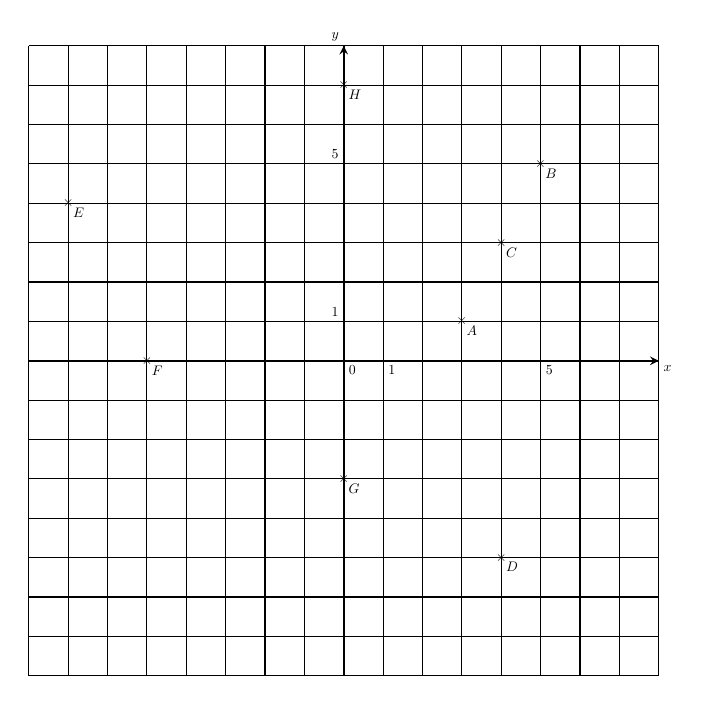
\begin{tikzpicture}[scale=0.5,every node/.style={scale=0.5}]
	%Points
	\coordinate(O)at(0,0);
	\coordinate(I)at(1,0);
	\coordinate(J)at(0,1);
	\coordinate(xstart)at(-8,0);
	\coordinate(xend)at(8,0);
	\coordinate(ystart)at(0,-8);
	\coordinate(yend)at(0,8);
	\coordinate(A)at(3,1);
	\coordinate(B)at(5,5);
	\coordinate(C)at(4,3);
	\coordinate(D)at(4,-5);
	\coordinate(E)at(-7,4);
	\coordinate(F)at(-5,0);
	\coordinate(G)at(0,-3);
	\coordinate(H)at(0,7);
	%Étiquettes
%	\draw (I) node[below right] {$1$};
%	\draw (J) node[above left] {$1$};
	\draw (xend) node[below right] {$x$};
	\draw (yend) node[above left] {$y$};	
	%%%%%%%%%%%%%%%%%%%%%%%%%%%%%%%%%%%%
	%Axes
	\draw [thick] (xstart) -- (xend);
	\draw [thick] (ystart) -- (yend);
	%Flèches
%	\draw [>=stealth,->] (O) -- (I);
%	\draw [>=stealth,->] (O) -- (J);
	\draw [>=stealth,->] (O) -- (xend);
	\draw [>=stealth,->] (O) -- (yend);
	%Grille
	\draw [thin] (-8,-8)grid(8,8);
	%%%%%%%%%%%%%%%%%%%%%%%%%%%%%%%%%%%%
	%étiquettes
	\foreach \point in {A, ..., H}
		\draw(\point)node{$\times$};
	\foreach \point in {A, ..., H}
		\draw(\point)node[below right]{$\point$};	
	\foreach \r in {0, 1, 5}
    	\draw[thick, below right] (\r,0) node{\r};
	\foreach \r in {1, 5}
    	\draw[thick, above left] (0,\r) node{\r};
\end{tikzpicture}
%}
\end{center}
\end{minipage}
\begin{minipage}{0.2\textwidth}
	\begin{enumerate}[]
		\item $A(~~~~~,~~~~~)$
		\item $B(~~~~~,~~~~~)$
		\item $C(~~~~~,~~~~~)$
		\item $D(~~~~~,~~~~~)$
		\item $E(~~~~~,~~~~~)$
		\item $F(~~~~~,~~~~~)$
		\item $G(~~~~~,~~~~~)$
		\item $H(~~~~~,~~~~~)$
	\end{enumerate}
\end{minipage}

\paragraph{Exercice~2} Placer un point connaissant ses coordonnées~:

\begin{minipage}{0.75\textwidth}
\begin{center}
%\fbox{
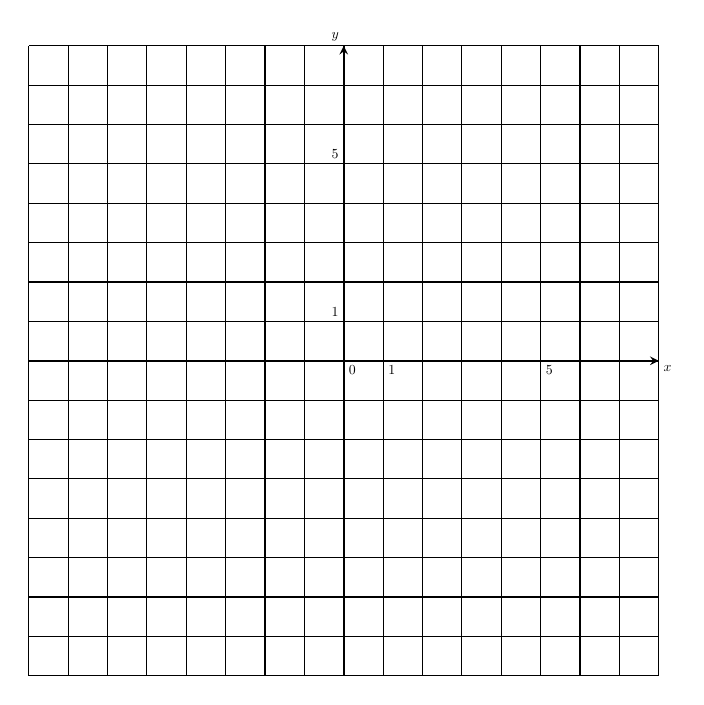
\begin{tikzpicture}[scale=0.5,every node/.style={scale=0.5}]
	%Points
	\coordinate(O)at(0,0);
	\coordinate(I)at(1,0);
	\coordinate(J)at(0,1);
	\coordinate(xstart)at(-8,0);
	\coordinate(xend)at(8,0);
	\coordinate(ystart)at(0,-8);
	\coordinate(yend)at(0,8);
	\coordinate(A)at(5,3);
	\coordinate(B)at(-2,3);
	\coordinate(C)at(-2,-4);
	\coordinate(D)at(6,2);
	\coordinate(E)at(7,-4);
	\coordinate(F)at(6,0);
	\coordinate(G)at(0,3);
	\coordinate(H)at(0,-7);
	%Étiquettes
%		\draw (I) node[below right] {$1$};
%		\draw (J) node[above left] {$1$};
	\draw (xend) node[below right] {$x$};
	\draw (yend) node[above left] {$y$};	
	%%%%%%%%%%%%%%%%%%%%%%%%%%%%%%%%%%%%
	%Axes
	\draw [thick] (xstart) -- (xend);
	\draw [thick] (ystart) -- (yend);
	%Flèches
%		\draw [>=stealth,->] (O) -- (I);
%		\draw [>=stealth,->] (O) -- (J);
	\draw [>=stealth,->] (O) -- (xend);
	\draw [>=stealth,->] (O) -- (yend);
	%Grille
	\draw [thin] (-8,-8)grid(8,8);
	%%%%%%%%%%%%%%%%%%%%%%%%%%%%%%%%%%%%
	%étiquettes
	
% Réponses
%	\foreach \point in {A, ..., H}
%		\draw(\point)node{$\times$};
%	\foreach \point in {A, ..., H}
%		\draw(\point)node[below right]{$\point$};
	
	\foreach \r in {0, 1, 5}
    	\draw[thick, below right] (\r,0) node{\r};
	\foreach \r in {1, 5}
    	\draw[thick, above left] (0,\r) node{\r};  
\end{tikzpicture}
%}
\end{center}
\end{minipage}
\begin{minipage}{0.2\textwidth}
	\begin{enumerate}[]
		\item $A(~~5~,~3~)$
		\item $B(~-2~,~3~)$
		\item $C(-2,-4)$
		\item $D(~~6~,~~2~)$
		\item $E(~~7~,~-4)$
		\item $F(~~6~,~~0~)$
		\item $G(~~0~,~~3~)$
		\item $H(~~0~,-7)$
	\end{enumerate}
\end{minipage}

\vspace{-2em}	

\end{minipage}
\end{document}
